\chapter{Malware}

Una definizione \textit{informale} può essere quella di programma \textbf{malevolo}, solitamente 
inserito di nascosto in un sistema, che ha lo scopo di compremettere la riservatezza, l'integrità o 
la disponibilità del sistema stesso.


\noindent I malware sono classificati in base a:
\begin{itemize}
    \item \textbf{Propagazione} (sw, rete, social engeneering, \dots)
    \item \textbf{Azioni sui dati} colpiti (corruzione, furto, crittografia, \dots)
    \item \textbf{Attack kit} (strumenti già pronti per attaccare)
    \item \textbf{Attori e/o motivazioni} dell'attacco
\end{itemize}

\begin{figure}[H]
    \centering
    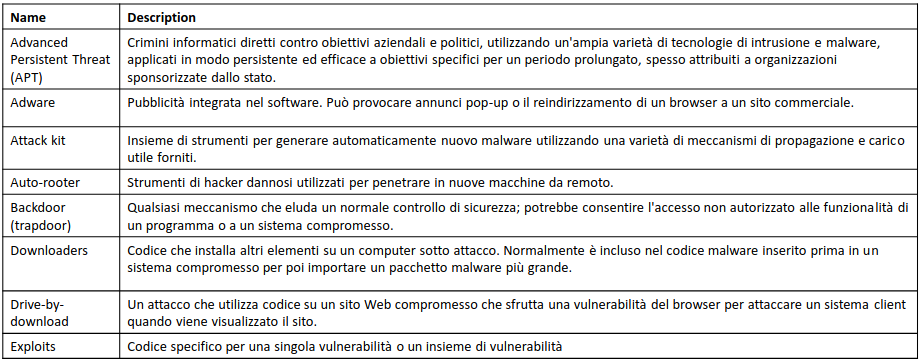
\includegraphics[width=1\linewidth]{chapters/5/images/classification1.png}
\end{figure}

\begin{figure}[H]
    \centering
    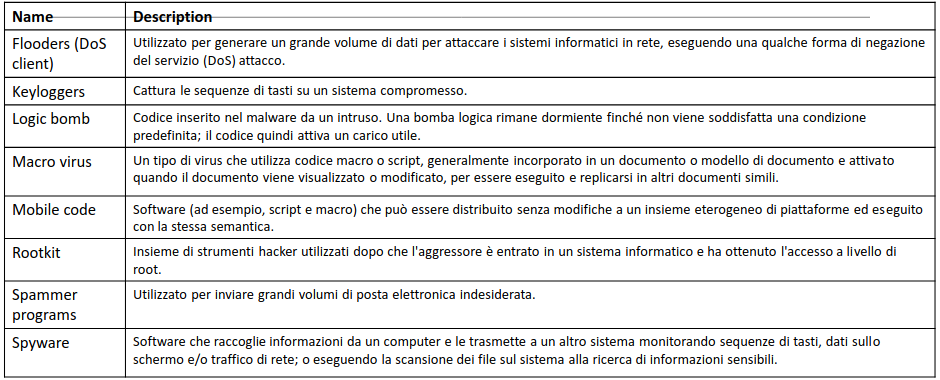
\includegraphics[width=1\linewidth]{chapters/5/images/classification2.png}
\end{figure}

\begin{figure}[H]
    \centering
    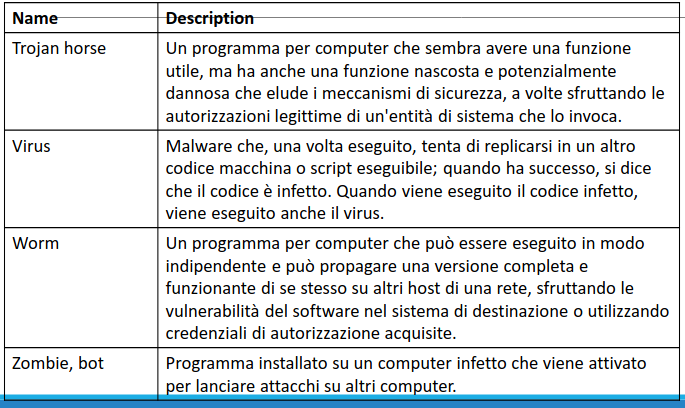
\includegraphics[width=1\linewidth]{chapters/5/images/classification3.png}
\end{figure}

\section{Trojan}
È un programma che ha un effetto evidente e atteso dall'utente, che ha però anche un 
effetto \textbf{nascosto} che viola le politiche di sicurezza e che viene condotto senza l'autorizzazione 
dell'utente

\section{Virus}
È un codice che può replicarsi modificando altri file o programmi per inserire codice in 
grado di replicarsi a sua volta; questa \textbf{proprietà di replicazione} è ciò distingue 
i virus dagli altri tipi di malware. Non svolge nessuna azione evidente, ma cerca di rimanere 
nell'ombra.

\noindent La replica richiede un certo tipo di assistenza da parte dell'utente, come ad esempio
cliccare su un allegato.

\noindent Un virus è composto da tre parti:
\begin{itemize}
    \item \textbf{Meccanismo di infezione}
    \item \textbf{Trigger:} evento che determina quando il payload viene attivato
    \item \textbf{Payload:} cosa fa il virus (oltre a diffondersi)
\end{itemize}

\noindent I virus attraversano quattro fasi:
\begin{enumerate}
    \item \textbf{Dormiente:} il virus è inattivo in attesa di essere attivato 
    \item \textbf{Scatenante:} il virus viene attivato 
    \item \textbf{Propagazione:} il virus inserisce una copia di sé stesso in certe parti del sistema; ogni programma 
    infetto conterrà ora un altro virus che entrerà a sua volta in fase di propagazione 
    \item \textbf{Esecutiva:} la funzione viene eseguita
\end{enumerate}

\subsection{Vettori di infezione}
I principali vettori di infezione sono:
\begin{itemize}
    \item \textbf{Boot sector} di dispositivi esterni; il codice è inserito nel boot sector e viene 
    eseguito in fase di avvio 
    \item \textbf{Eseguibili}
    \item \textbf{File macro:} il virus si attacca ai documenti per propagarsi 
\end{itemize}

\subsection{Classificazione dei virus}
È possibile classificare i virus in base alle \textbf{tecniche usate per superare i controlli 
di sistema:}
\begin{itemize}
    \item \textbf{Cifratura del virus:} crea una chiave per \textit{"crittografarsi"}; quando viene 
    chiamato un programma infetto, con tale chiave viene decifrato il virus. Per evitare pattern 
    di bit, durante la propagazione la chiave viene cambiata
    \item \textbf{Stealth virus:} si nasconde dal rilevamento da parte dell'antivirus, tramite mutazione 
    o compressione del codice 
    \item \textbf{Polymorphic virus:} durante la replica crea copie che svolgono la stessa funzione 
    ma che hanno pattern di bit diversi 
    \item \textbf{Metamorphic virus:} si riscrive completamente ad ogni iterazione per aumentare la 
    difficoltà di rilevamento
    \item \textbf{Compression virus:} comprimono il file eseguibile in modo che la versione infetta 
    abbia la stessa dimensione di quella originale
\end{itemize} 

\section{Worm}
I worm sono programmi \textit{stand alone} (a differenza dei virus che devono essere attivati 
da un qualche evento) in grado di replicarsi.

\noindent Le fasi di esecuzione sono:
\begin{itemize}
    \item \textbf{Probing:} cerca informazioni sulla macchina 
    \item \textbf{Expoloitation:} sfrutta le informazioni raccolte per trovare vulnerabilità
    \item \textbf{Replicazione}
    \item \textbf{Attacco} (payload)
\end{itemize}

\section{Drive-by-download}
Sfruttano \textbf{vulnerabilità del browser} per installare codice malevolo ad insaputa dell'utente 
nel momento in cui visita la pagina web dell'attaccante. 

\section{Clickjacking}
L'attaccante intercetta un \textit{click} dell'utente per costringerlo a fare delle cose 
contro la sua volontà.

\section{Zombie e botnet}
Lo \textit{zombie} è una singola macchina, mentre la \textit{botnet} è un insieme di macchine 
zombie controllate da una singola entità; vengono usate per fare DDoS, phishing, spamming, \dots

\section{Rootkit}
È un insieme di programmi installati su un sistema per mantenere l'accesso ad un sistema, ad 
esempio, con privilegi di amministratore, nascondendo le prove della sua presenza e aggirando 
i meccanismi di controllo.

\noindent Permettono di fare attacchi anche con scarse conoscenze tecniche.

\section{Scareware}
Software che hanno lo scopo di diffondere shock, ansia e/o la percezione di una minaccia; sono 
un attacco di \textit{social engeneering}.

\section{Ransomware}
Software che tiene in ostaggio il sistema per richiedere un riscatto all'utente, spesso tramite
cifratura.

\section{Vulnerabilità zero-day}
Si intende un'exploit non ancora nota e che non ha quindi una contromisura.

\section{Spear phishing}
Viene \textbf{studiato nel dettaglio il bersaglio}, in modo tale da fare del phishing più mirato 
ed efficace.

\section{Spyware}
Malware che raccoglie piccole informazioni alla volta sugli utenti a loro insaputa,
come ad esempio un \textit{keylogger}.

\section{APT - Advanced Persistent Threats}
\begin{itemize}
    \item \textit{\textbf{Advanced:}} è un'applicazione con un ampia varietà di tecnologie di intrusione e malware
    \item \textit{\textbf{Persistent:}}
    attacchi per un periodo di tempo prolungato verso il target
    \item \textit{\textbf{Target:}} target selezionati in modo accurato
\end{itemize}

\noindent Le fasi principali di un attacco tramite APT sono:
\begin{itemize}
    \item \textbf{Ricognizione:} si sceglie una vittima e la si studia 
    \item \textbf{Weaponization:} si mette un trojan che permette accesso remoto in un payload consegnabile (email, USB, web)
    \item \textbf{Sfruttamento:} il codice malevolo viene attivato per portare a termine il suo scopo
\end{itemize}


\newpage
\section{Approcci alle contromisure per i malware}
Le principali contromisure da adottare sono:
\begin{itemize}
    \item assicurare di \textbf{aggiornare} tutti i sistemi
    \item ridurre al \textbf{minimo le vulnerabilità}
    \item impostare adeguati \textbf{controlli} di accesso alle applicazioni e ai dati 
    \item \textbf{limitare} il numero di file a cui un utente può accedere, e che quindi può 
    potenzialmente infettare
\end{itemize}

\noindent Le azioni da prendere nel caso il sistema venga attaccato sono:
\begin{itemize}
    \item \textbf{Rilevamento:} accertarsi della presenza del virus; può essere fatto con:
    \begin{itemize}
        \item programmi anti-virus, 4 generazioni:
        \begin{itemize}
            \item \textbf{scanner semplici} $\rightarrow$ ricercano malware noti 
            \item \textbf{scanner euristici} $\rightarrow$ utilizzano regole euristiche
            \item \textbf{trap di attività:} viene cercato il malware in base alle sue azioni piuttosto che in base alla sua 
            struttura $\rightarrow$ l'analisi è dinamica 
            \item \textbf{protezione completa:} più tecniche usate insieme 
        \end{itemize}
        \item meccanismi di protezione perimetrale nei firewall
    \end{itemize}
    \item \textbf{Identificazione:} individuare lo specifico malware
    \item \textbf{Rimozione} di tutte le tracce dal sistema
\end{itemize}









